\label{sec:5.3}
%\clearpage
%%%%%%%%%%%%%%%%%%%%%%%%%%%%%%%%%%%%%%%%%%%%%%%%%%%%%%%
%(Prakash/Grace) Discuss ADC Core linearity
%%%%%%%%%%%%%%%%%%%%%%%%%%%%%%%%%%%%%%%%%%%%%%%%%%%%%%%
The measured ADC INL of the Cold ADC is approximately 1 LSB at a 12-bit level. However, simulations suggest 0.5 LSB INL after calibration is possible. The key reasons for the discrepancy are the lack of corner models at cold and the Monte Carlo analysis done using the warm models was insufficient. Testing indicates the ADC linearity is limited primarily by insufficient op-amp gain in the stages. Since the calibration algorithm can only correct linear gain error, higher-order non-linearity beyond what was expected limited the performance. The op-amp becomes nonlinear as their swing increases because the output resistance of the devices connected to the output decreases when the voltage across them is reduced. This is a known issue and was mitigated in the design by increasing the open-loop gain. The main suspect in the reduced linearity is that the raw open-loop gain is lower than expected and therefore the closed-loop rejection of the non-linearity is not good enough. To verify the large closed-loop gain non-linearity in the stages, we adjusted the reference voltages to reduce the dynamic range of each stage and this improved the linearity, as it should if the nonlinearity steps from the output stages of the op-amps. This is demonstrated in Figure~\ref{fig:linearity_100mv} and~\ref{fig:linearity_200mv}. In Figure~\ref{fig:linearity_100mv}, the differential reference is reduce 100 mV from nominal, and in Figure~\ref{fig:linearity_200mv} the differential reference is reduced 200 mV from nominal. Comparing Figures~\ref{fig:linearity_100mv} and \ref{fig:linearity_200mv}, the DNL is improved and becomes more uniform as the reference is reduced. 

\begin{figure}[h!]
\centering
  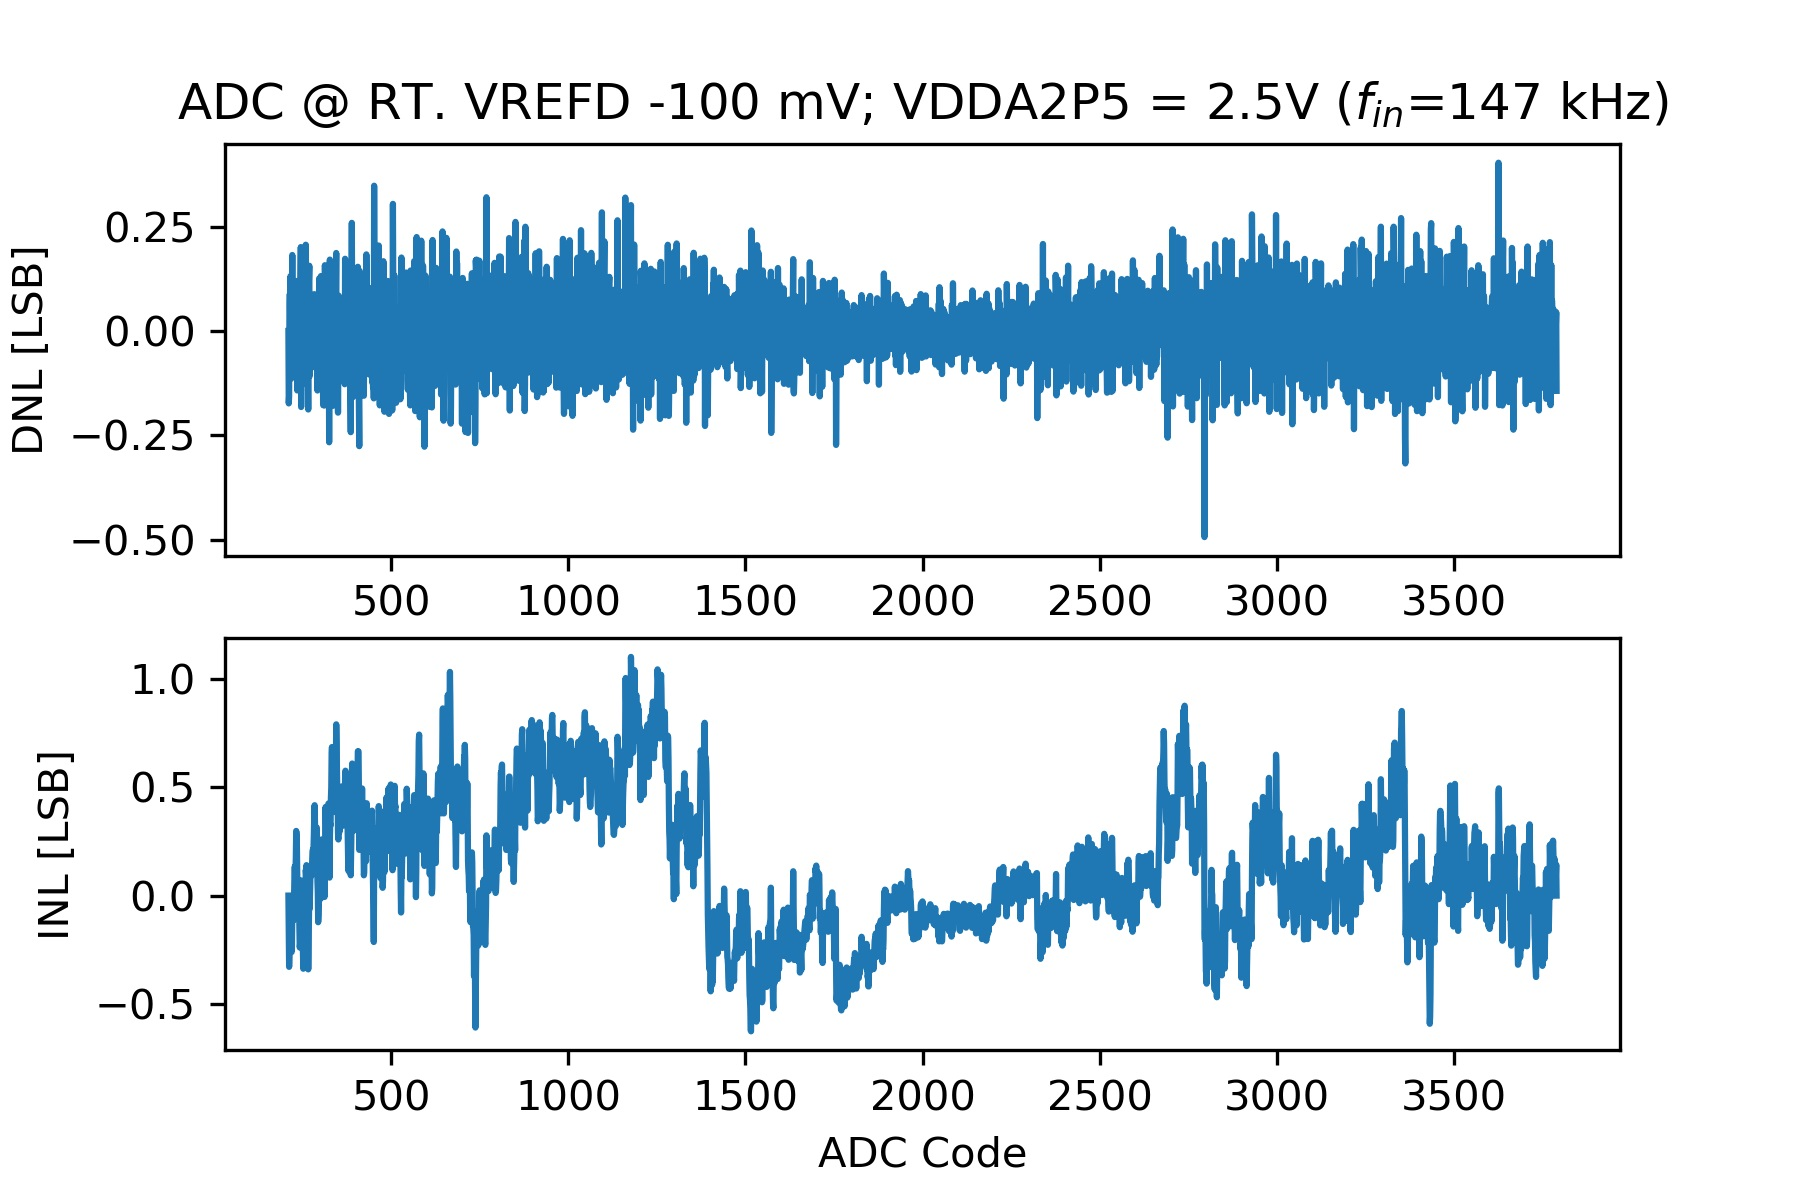
\includegraphics[width=0.7\linewidth]{figures/prakash_fig/linearity_100mv.JPG}
  \caption{ADC linearity with VREFN/P +/- 100mV}
  \label{fig:linearity_100mv}
\end{figure}

\begin{figure}[h!]
\centering
  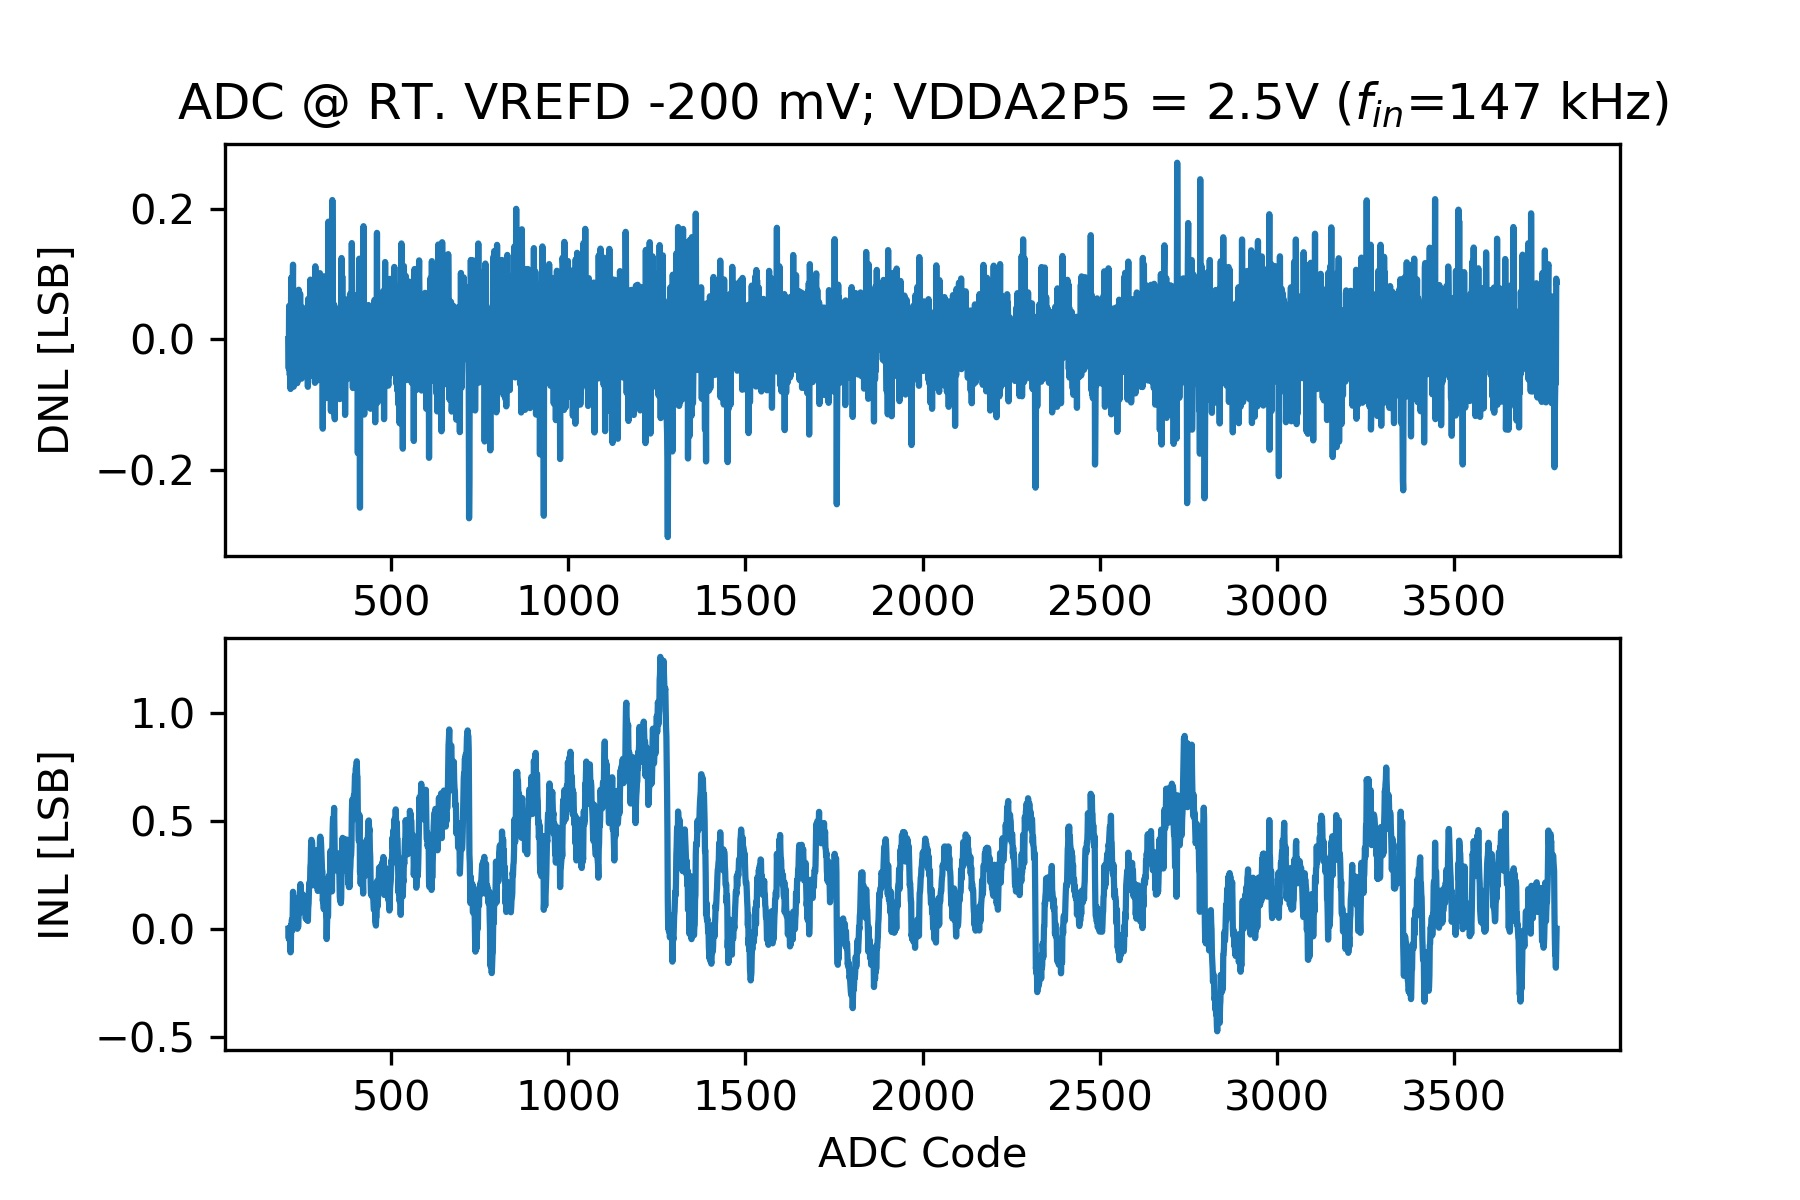
\includegraphics[width=0.7\linewidth]{figures/prakash_fig/linearity_200mv.JPG}
  \caption{ADC linearity with VREFN/P +/- 200mV}
  \label{fig:linearity_200mv}
\end{figure}

%\begin{figure}[h!]
%\centering
%  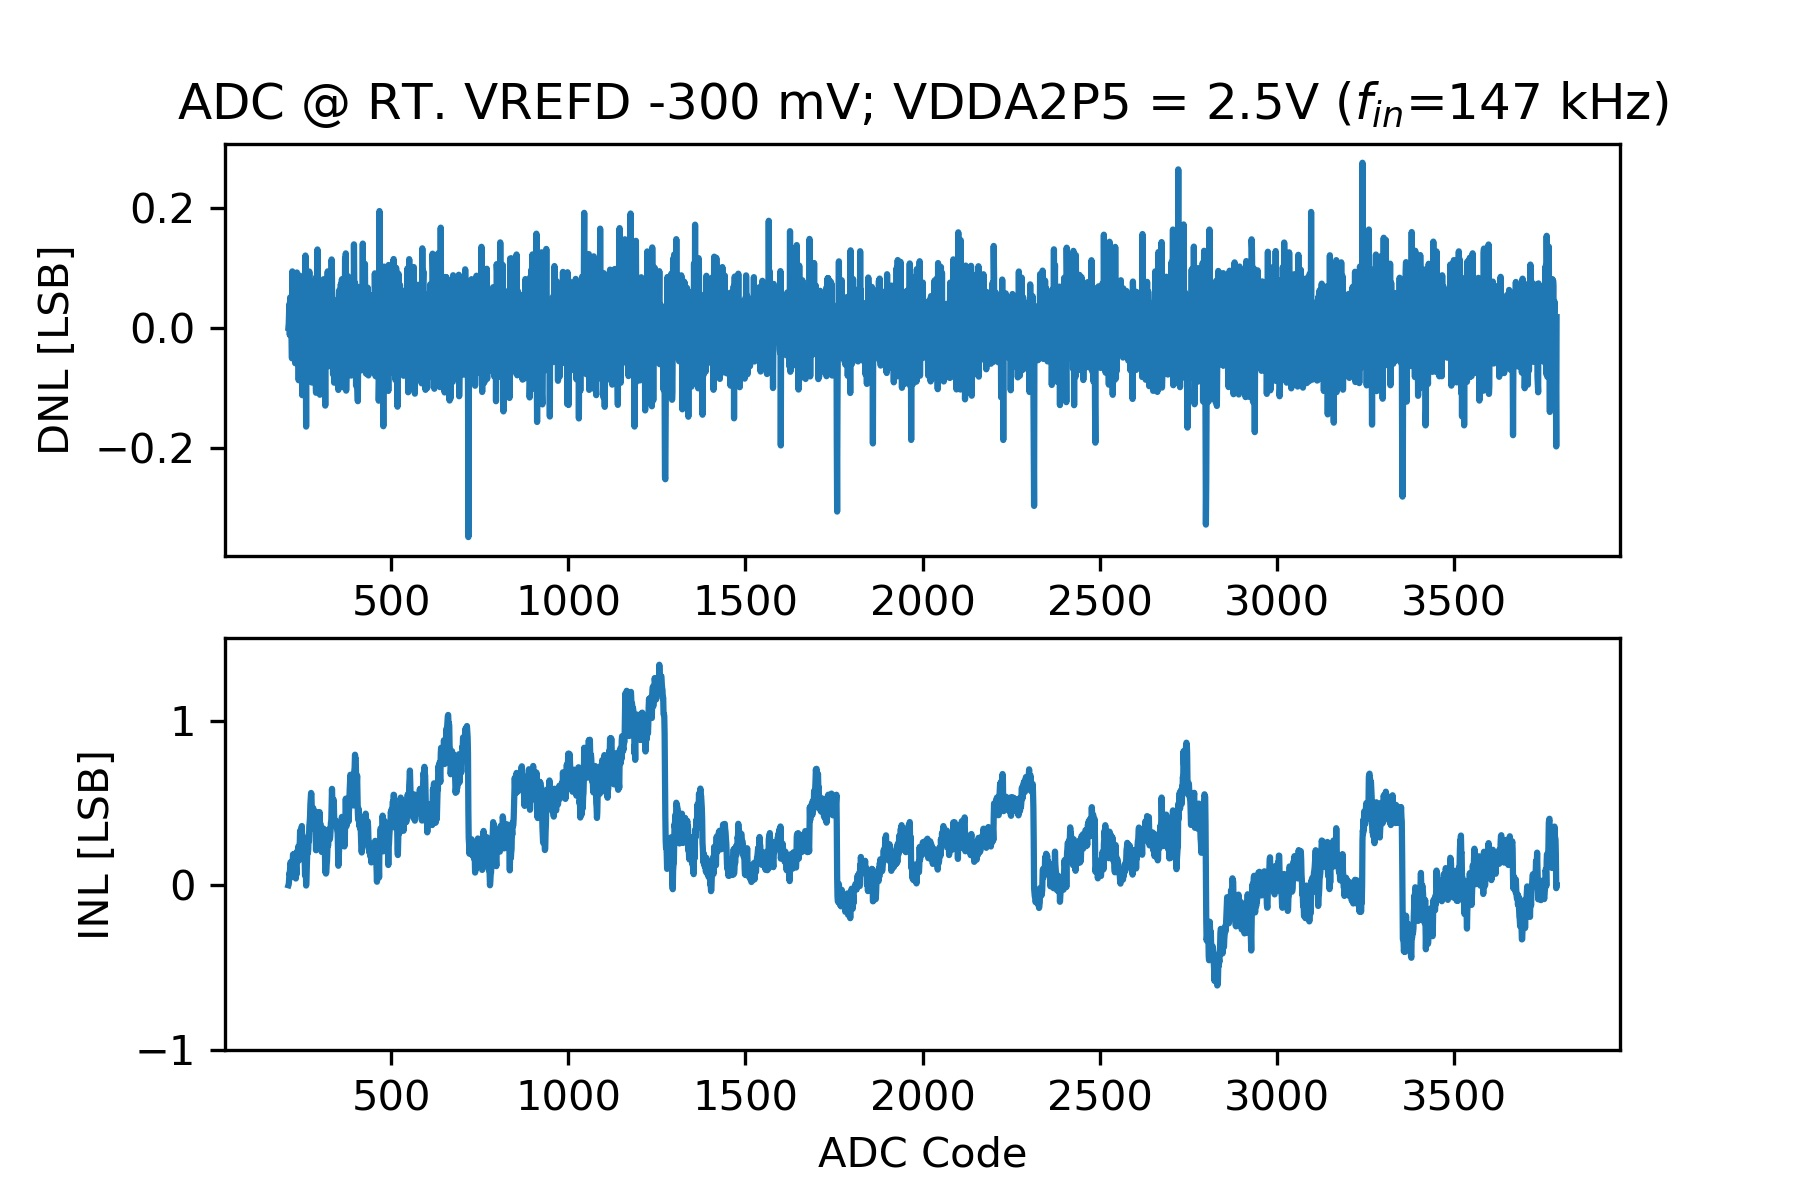
\includegraphics[width=0.7\linewidth]{figures/prakash_fig/linearity_300mv.JPG}
%  \caption{ADC linearity with VREFN/P +/- 300mV}
%  \label{fig:linearity_300mv}
%\end{figure}

To get evidence about what is the root cause of the increased linearity, we can use the programmability of the ColdADC to run various experiments to rule out potential causes. To rule out that the observed nonlinearity was caused by incomplete stage settling, we first operated the ADC with increased bias currents, to reduce settling time. This did not improve performance. We then slowed down the ADC by a factor of 16 and reduced the op-amp bias currents. Reducing the bias currents has the effect of increasing the op-loop gain, but also slows down the circuit, necessitating the reduced sampling rate. 
The results of this experiment is shown in Figure~\ref{fig:linearity_GB_ON}. The ColdADC demonstrates superior performance in this situation, strongly suggesting the increased open-loop gain mitigates the gain-drooping caused by the op-amp output resistance. Note that the references are nominal here, showing that the observed nonlinearity it reduced in this case by the negative feedback.

\begin{figure}[h!]
\centering
  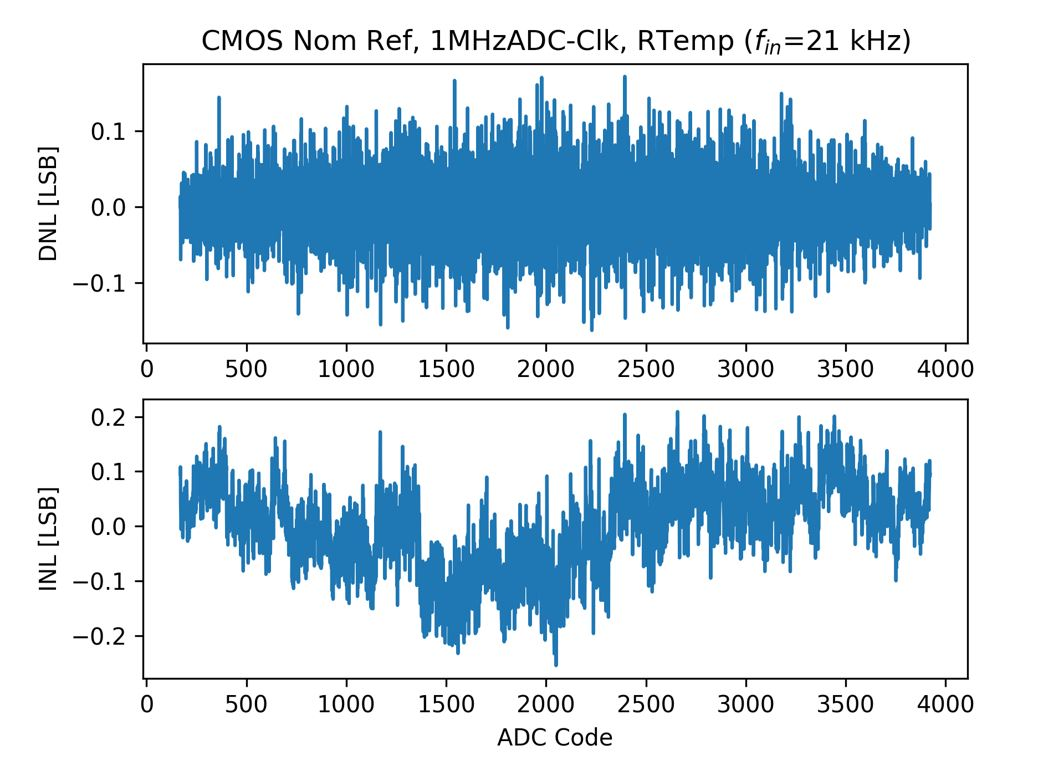
\includegraphics[width=0.7\linewidth]{figures/prakash_fig/linearity_GB_ON.JPG}
  \caption{Linearity with Gain Boosters ON}
  \label{fig:linearity_GB_ON}
\end{figure}

A schematic of the op-amp used in the ADC stages is shown in Figure~\ref{fig:op_amp_1}. The circuit uses a standard folded-cascode topology with gain boosting amplifiers used to increase the open-loop gain. These gain boosting amplifiers work by regulating the voltage drop across the output transistors, increasing their output resistance. Simulations suggested that the gain boosting amplifiers increased the open-loop gain of the op-amp by approximately a factor of 5 (14 dB).

\begin{figure}[h!]
\centering
  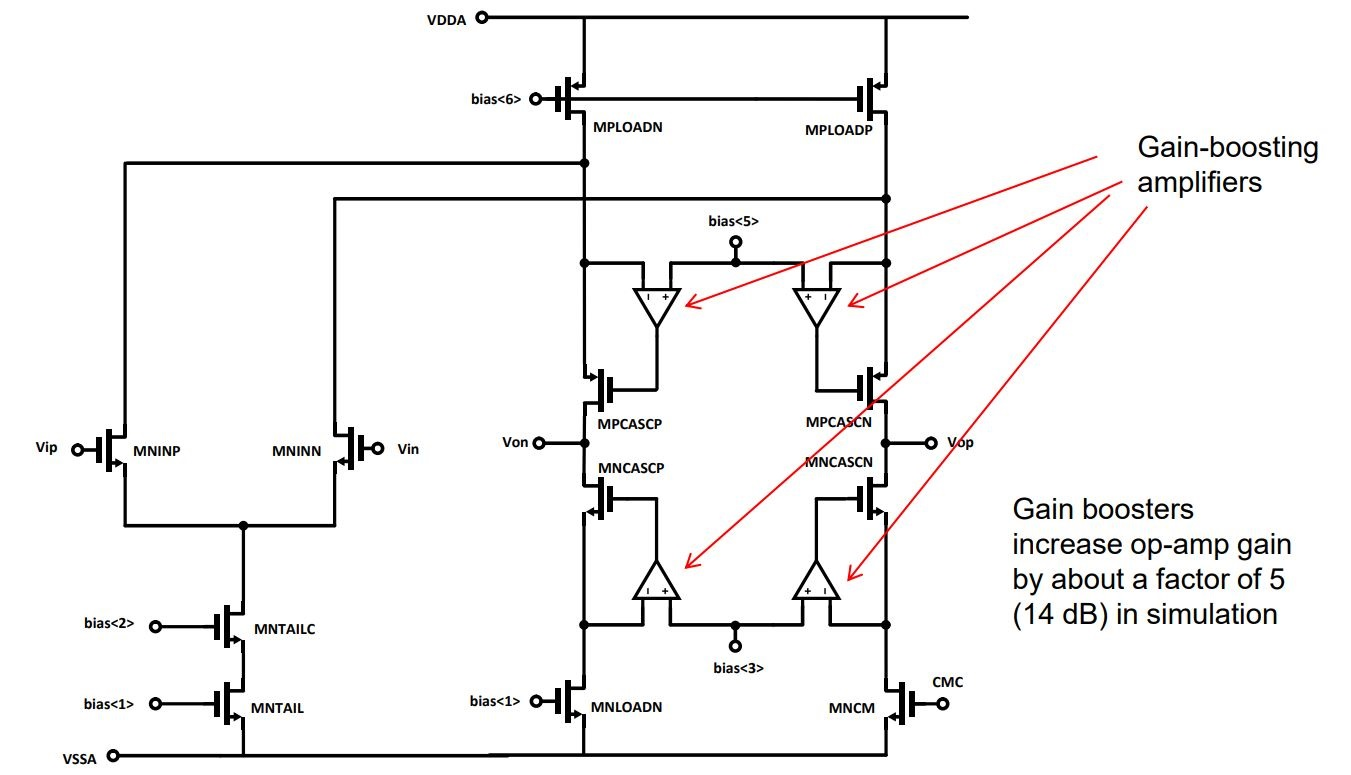
\includegraphics[width=0.9\linewidth]{figures/prakash_fig/op_amp.JPG}
  \caption{Op-Amp used in ColdADC stages.}
  \label{fig:op_amp_1}
\end{figure}

To narrow down what precisely in the op-amp was causing the lower-than-expected gain, we disabled the gain boosting amplifiers. This is possible to do through the configuration interface and was included for debugging purposes. When we disabled the gain boosting amplifiers, but held all other conditions constant, the linearity degraded as shown in Figure~\ref{fig:linearity_GB_OFF}. In fact, the INL increased by over a factor of 2 and the DNL increased as well.


\begin{figure}[h!]
\centering
  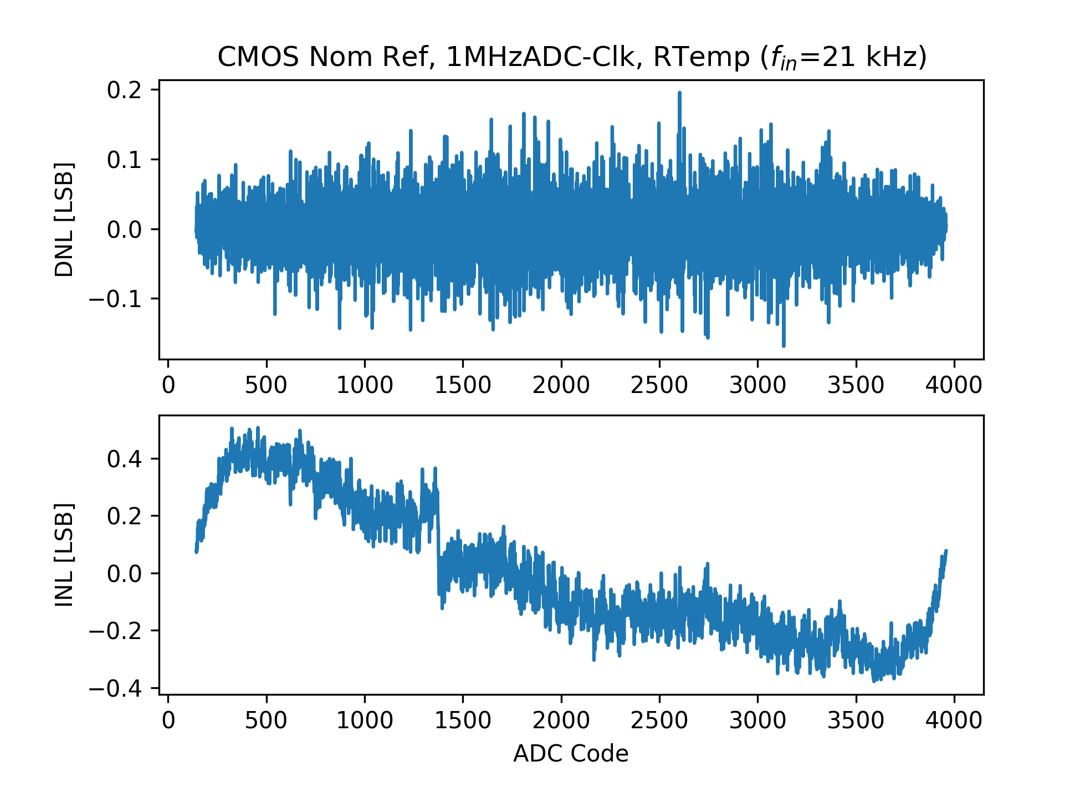
\includegraphics[width=0.7\linewidth]{figures/prakash_fig/linearity_GB_OFF.JPG}
  \caption{Linearity with Gain Boosters OFF.}
  \label{fig:linearity_GB_OFF}
\end{figure}

For further evidence, we modeled the ADC behaviorally using MATLAB. The simulated linearity obtained after setting the op-amp open-loop gain in the model to 80 dB is shown in Figure~\ref{fig:behav_GB_ON}, which is a result similar to Figure~\ref{fig:linearity_GB_ON}. By reducing the open-loop gain to 74 dB, we obtained the result in Figure~\ref{fig:behav_GB_OFF} which closely follows the linearity structure of Figure~\ref{fig:linearity_GB_OFF}. This gives further evidence the issue is insufficient gain in the gain boosting amplifiers. Based on the behavioral modeling, we estimate the gain-boosting amplifiers are providing approximately 6 dB in additional gain, rather than the 14 dB that was expected.
\begin{figure}[h!]
\centering
  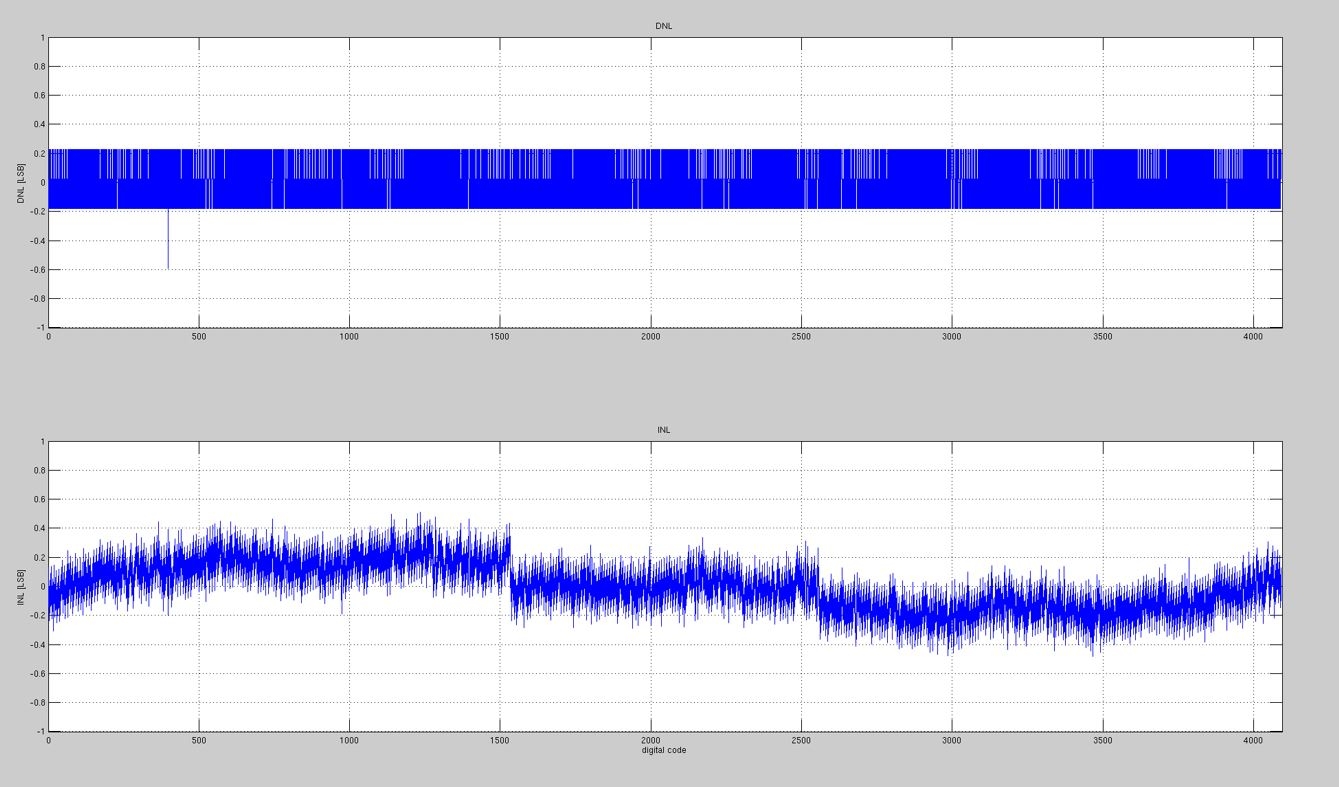
\includegraphics[width=0.7\linewidth]{figures/prakash_fig/behav_GB_ON.JPG}
  \caption{MATLAB model - gain boosters on -> 80 dB op-amp gain.}
  \label{fig:behav_GB_ON}
\end{figure}

\begin{figure}[h!]
\centering
  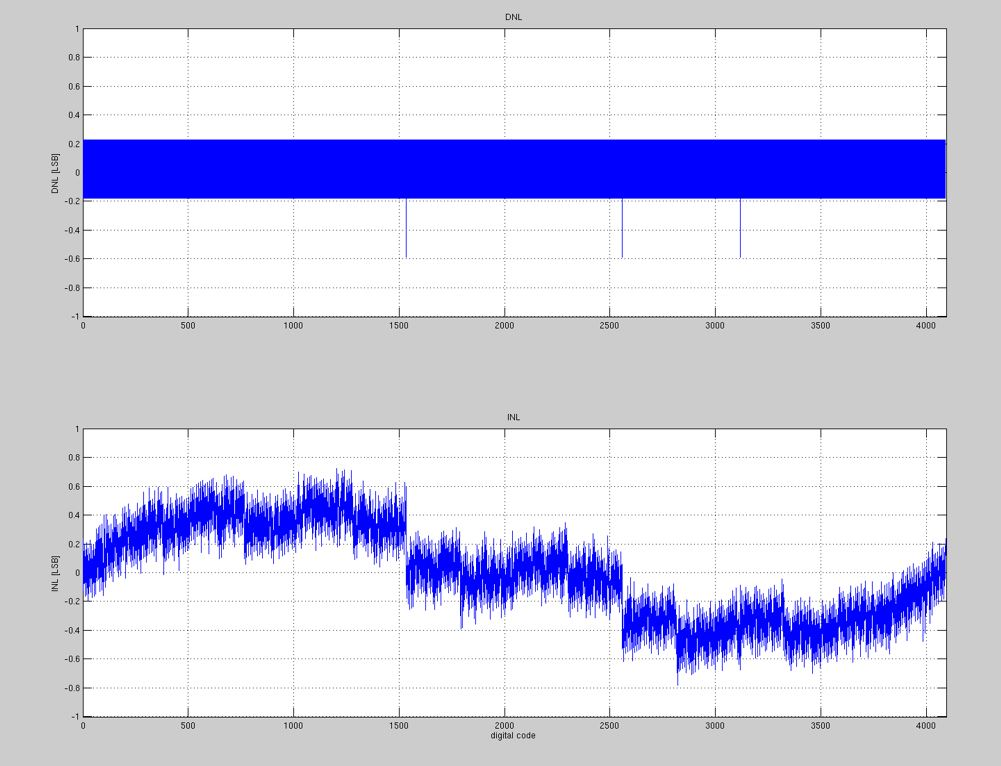
\includegraphics[width=0.7\linewidth]{figures/prakash_fig/behav_GB_OFF.JPG}
  \caption{MATLAB model - gain boosters off -> 74 dB op-amp gain.}
  \label{fig:behav_GB_OFF}
\end{figure}
Analysis of the circuits in the gain-boosting amplifiers indicates that they may have insufficient design margin in their biasing networks. The gain-boosting amplifiers and op-amp can be improved by redesigning them to better center their operating points across process and temperature.

Corner analysis of the complete op-amp before and after the gain-boosting redesign is shown in Figures~\ref{fig:opamp_gain_rt} and \ref{fig:opamp_gain_m_rt}, respectively. While the corners are only strictly valid at room temperature, the take away here is that the minimum open-loop gain across corners after the redesign is higher than the maximum open-loop gain before redesign. The design fix is being finalized and will soon be implemented in the layout.

\begin{figure}[h!]
\centering
  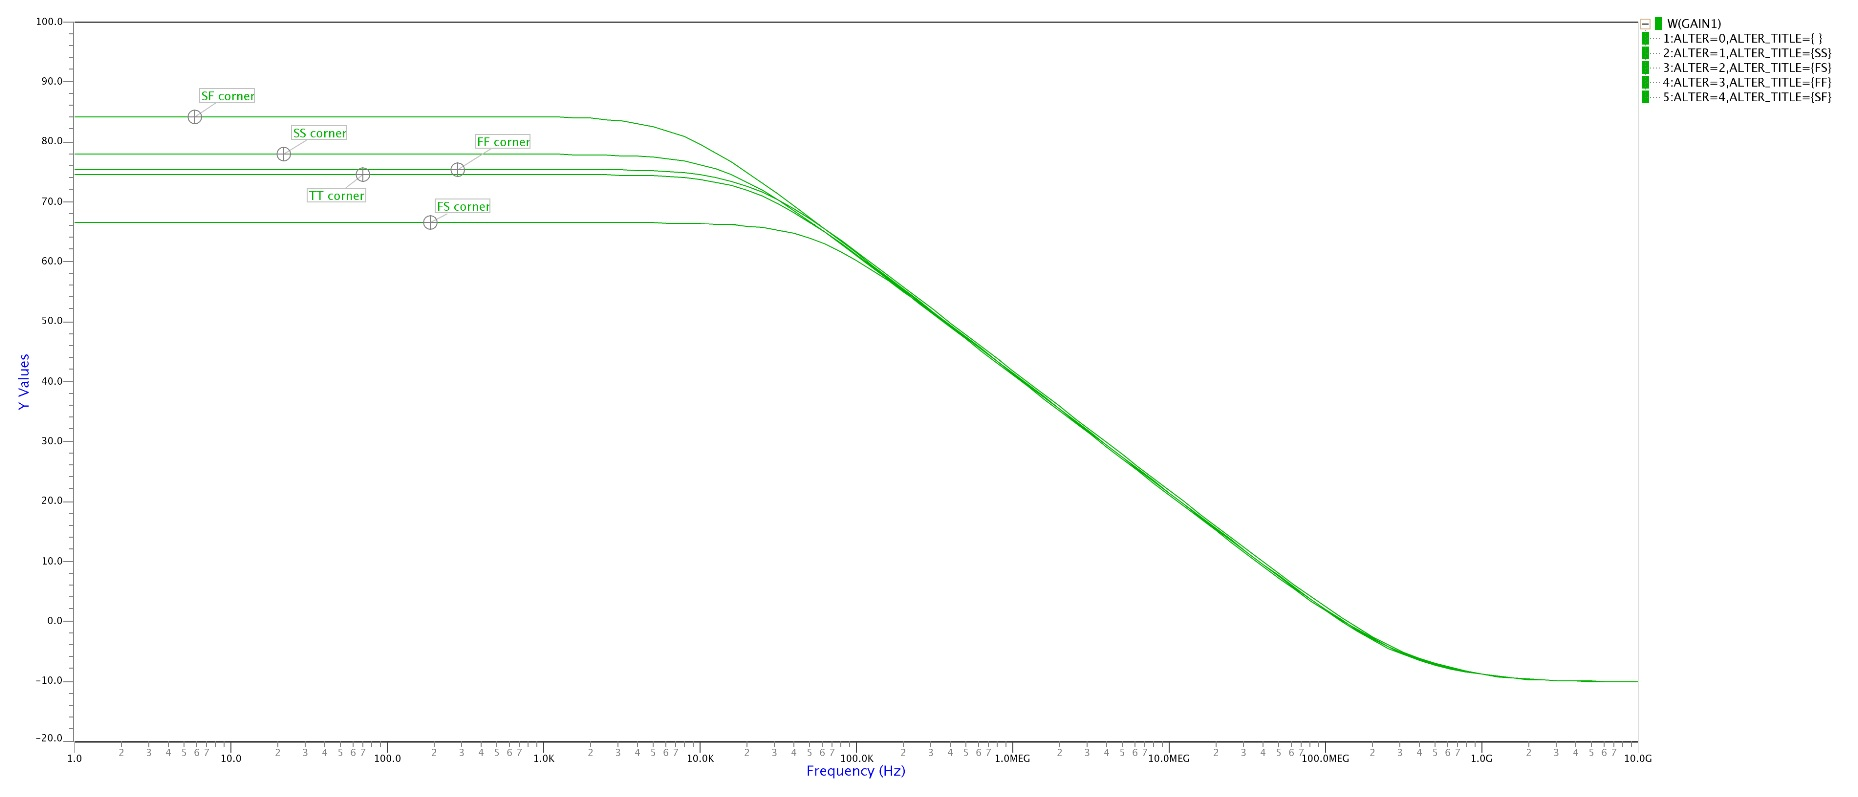
\includegraphics[width=0.8\linewidth]{figures/prakash_fig/opamp_gain_rt.JPG}
  \caption{Corner analysis of the op-amp gain, with current gain booster circuit.}
  \label{fig:opamp_gain_rt}
\end{figure}

\begin{figure}[h!]
\centering
  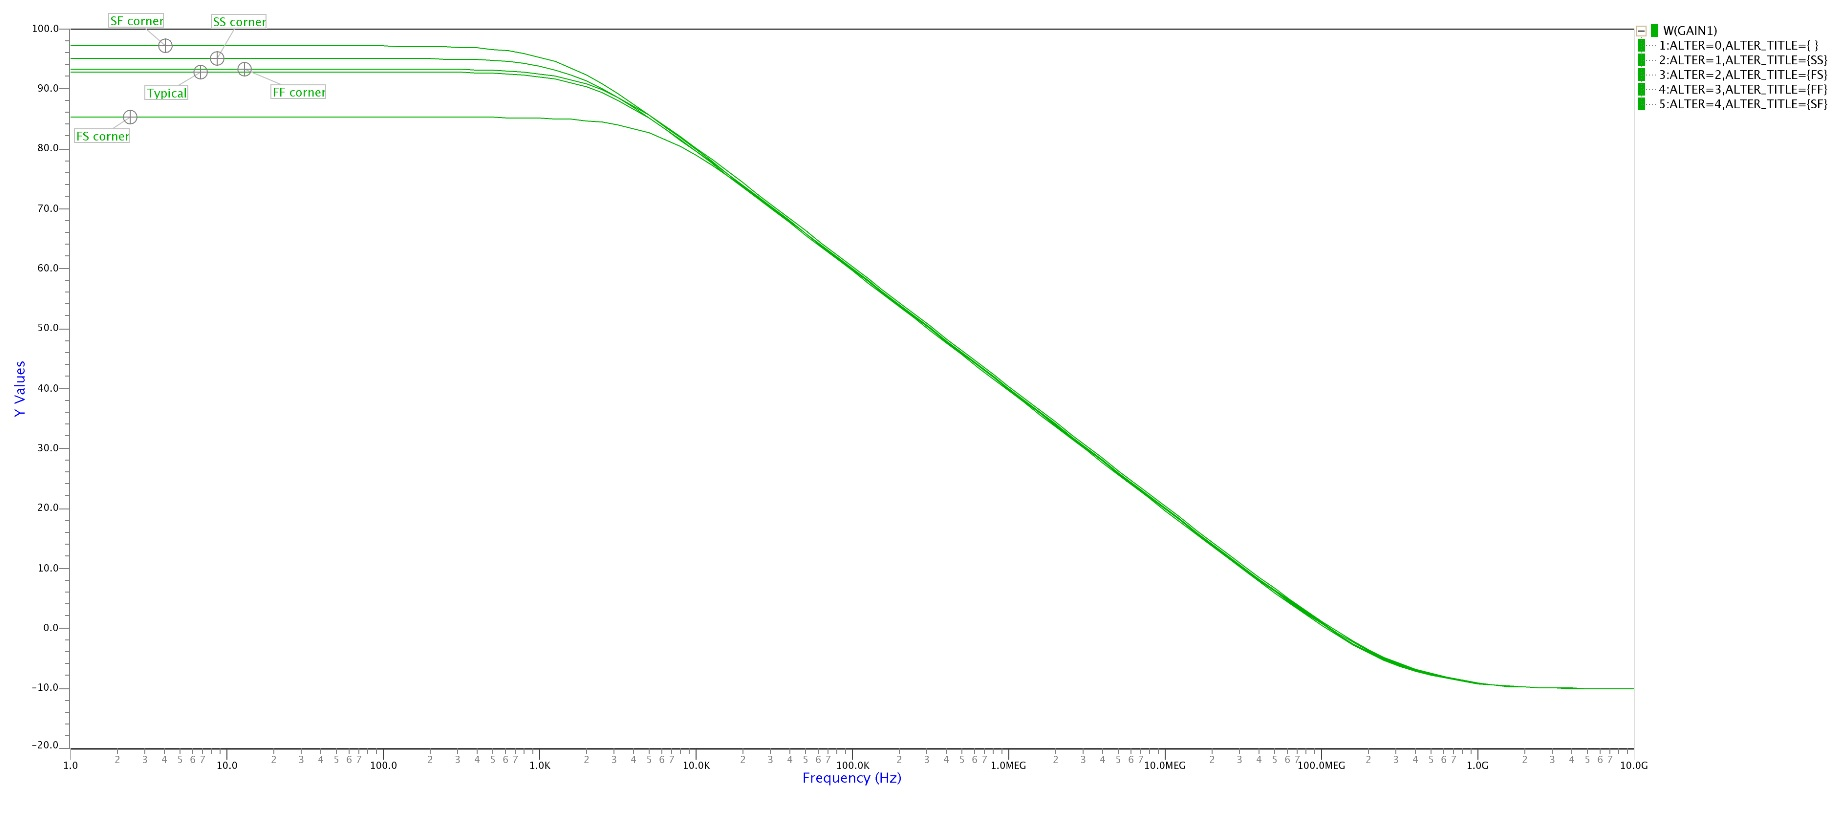
\includegraphics[width=0.8\linewidth]{figures/prakash_fig/opamp_gain_m_rt.JPG}
  \caption{Corner analysis of the op-amp gain, with improved gain booster circuit.}
  \label{fig:opamp_gain_m_rt}
\end{figure}

